%%%%%%%%%%%%%%%%%%%%%%%%%%%%%%%%%%%%%
\chapter{Standard Model and Rare Z and Higgs decays to quarkonia}
\label{chaptertheory}

\section{Standard Model and Local Gauge Invariance}
\label{section_sm}

% The human quest for understanding the Universe, goes through taking a complex problem and break it down into smaller (simpler) ideas, that, when stacked together, gives rise to a proper explanation of a phenomenon and, in the best scenario, allows us to make predictions about unexpected or less known aspects of subject. The Standard Model (SM) embodies this idea and attempts not only to explain the Universe in fundamental process (interactions), but also in terms of fundamentals components (particles). To what it proposes to explain, the Standard Model have been proven very effective.
 
Physics understands the matter and how it interacts in terms of two components: four fundamentals forces and elementary particles. From the weakest to the strongest, the fundamental forces are: gravitational, weak, electromagnetic and strong. All share common characteristics like, being mediated by particles~\footnote{There is no evidence of the existence of the Graviton (force carrier associated to the gravitational force), even though, it is theorized by models that wish to comprehend gravity in a quantum perspective.}, being relevant within some effective range and have a associate a charge-like quantity (i.e. intrinsic characteristic of the object) that defines whether or not, particles might be subjected to a specific interaction.

Along with the fundamental interactions, the Standard Model (or simply \textit{SM}) defines every existing matter in the Universe as a set of fundamental quantum objects, with properties that define their interaction. Those objects are said to be fundamental since, in the context of the SM, they are the smallest possible components of matter. We shall refer to them as fundamental particles. There four of those mediating particles (force carriers), gluon ($g$ - for the strong interaction), photon ($\gamma$ - for the electromagnetic interaction), Z and W (for weak interaction), all of them being vector bosons (spin 1). Besides the interaction mediators, described at Table~\ref{fundamental_forces}, the fundamental particles are divided in two groups (\textit{quarks} and \textit{leptons}), with three generations, each. These are not force carriers, but elementary particles, endowed with charge-like characteristics that allow them to by exchange the vector bosons. Those are the building blocks of Matter in our Universe.

Figure~\ref{sm_summary} summarizes their properties. Table~\ref{fundamental_forces} presents the relative strength and effective range, for each on of the four fundamental interactions. The gravitational force is not study subject of the Standard Model.

\begin{figure}[!htbp]
  \begin{center}
  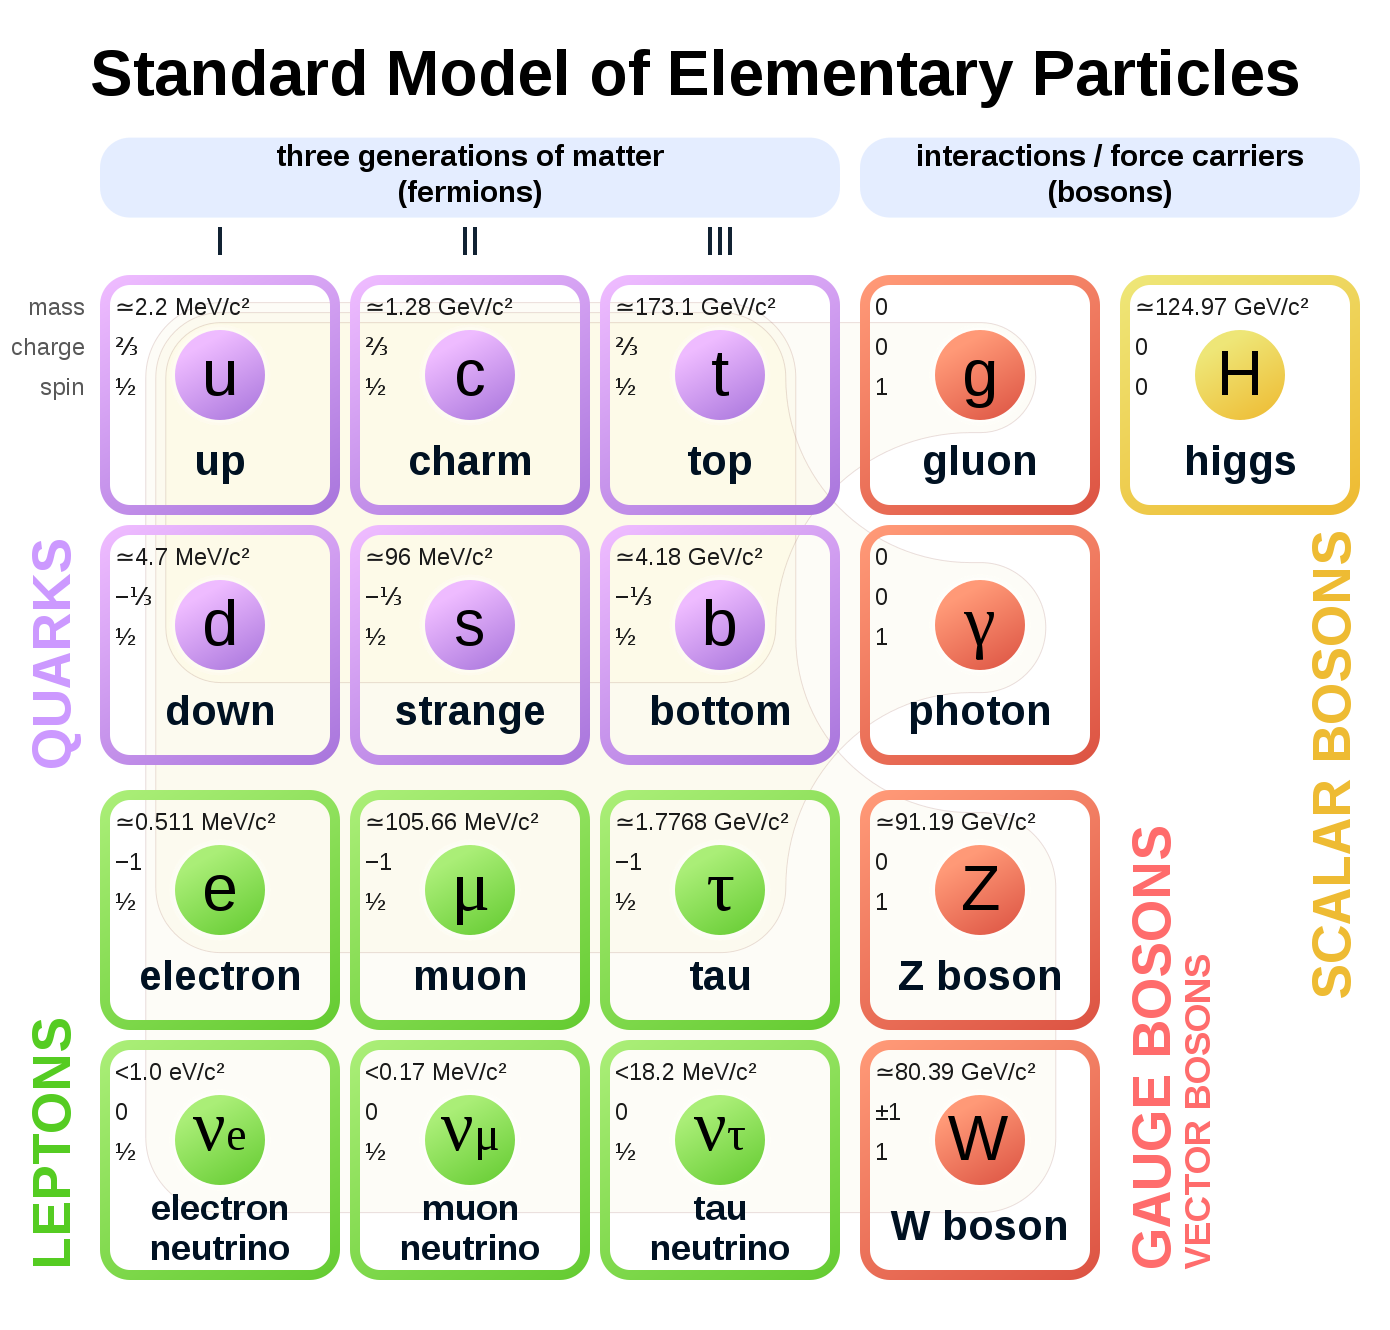
\includegraphics[width=0.6\textwidth ]{figures_and_tables/theory/sm.png}
  \end{center}\vspace*{-.5cm}
  \caption{Elementary particles of the Standard Model, with their masses charges and spin. Those particles can be divided in two classes: boson (the interaction/force carriers) and the fermions, which are divided in three generations. Source:~\cite{fig_sm_summary}.}
  \label{sm_summary}
  \end{figure}
 

\begin{table}[htp]
  \begin{center}
      \caption{Relative strength (with respect to the strong force) and effective range of action for the four fundamentals interactions.}
    \begin{tabular}{ cccc }
       & Mediator & Relative Strength & Effective Range \\ \hline
      Gravitational & Graviton & $10^{-41}$ & $\infty$ \\ 
      Weak & W and Z bosons & $10^{-16}$ & $10^{-18}$ m \\ 
      Electromagnetic & Photon & $10^{-3}$ & $\infty$ \\ 
      Strong & gluons & $1$ & $10^{-15}$ m\\ \hline
      \end{tabular}
  \label{fundamental_forces}
  \end{center} 
  \end{table}


There are six quark, up and down ($u$ and $d$ - first generation), charm and strange ($c$ and $s$ - second generation), top and bottom ($t$ and $b$ - first generation), in increasing invariant mass order of the generations. Since they interact thought all the three fundamental forces of the SM, they are said to possess electrical charge, flavour and color. Their generational counterparts, the leptons, don't interact via strong interaction, that is why they are said to have only flavours and electric charge. The leptons are electron and electron neutrino ($e$ and $\nu_e$ - first generation), muon and muon neutrino ($\mu$ and $\nu_{\mu}$ - second generation) and tau and tau neutrino ($\tau$ and $\nu_{\tau}$ - third generation). The neutrinos, within the SM, are massless, even though, experimental measurements have shown that they actually have mass~\cite{Patrignani:2016xqp}. Neutrinos are also electrically neutral, meaning that they only interact through weak interactions.

Figure~\ref{sm_summary} also presents the Higgs Boson ($H$) which is part of the SM and shall be discussed later.

Within the Standard Model, the theoretical basis that describe the fundamental interactions are derived from a common principle: the local gauge invariance. According to Salam and Ward~\cite{ward_salam}:


\begin{quote}
  "Our basic postulate is that it should be possible to generate strong, weak and electro-magnetic interaction terms [...], by making local gauge transformations on the kinetic-energy terms in the free Lagrangian for all particles."
\end{quote}

Taking the Quantum Electrodynamics (QED) as an example: the quantum field theory that describes the x


The fundamental theories that compose the Standard Model are all derived from a fundamental principle call 

The electromagnetic force, in the context of fundamental interactions, is describe by a gauge theory called quantum electrodynamics. 




\todo{Electroweak} 



